\newpage
\section{Pascal's Pyramid}\label{A:pyramid}

A \textit{pyramid} is a three-dimensional object that has some polygon
as its base and triangles that converge to a point as its sides. Fancy
folks call a triangular-based pyramid a
\textit{tetrahedron}.\index{tetrahedron}
\[
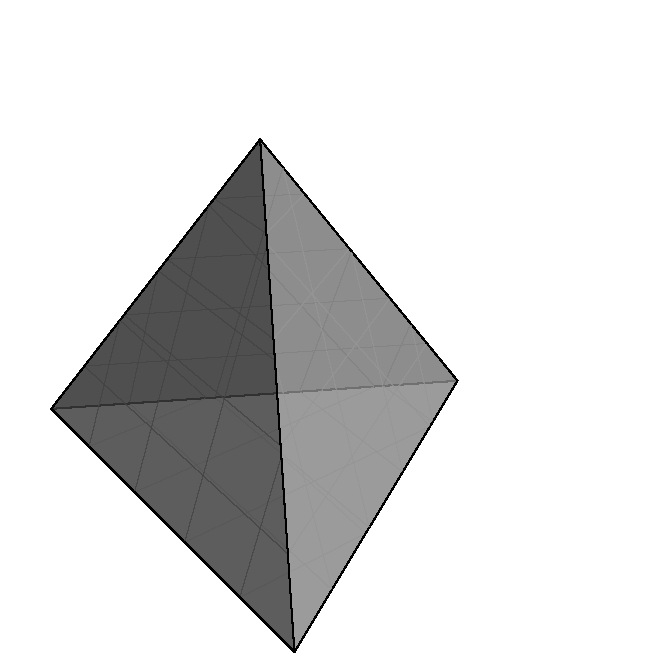
\includegraphics[scale=.5]{../graphics/pyr.pdf}
\]
Since three-dimensional objects are hard to view on a flat sheet of
paper, sometimes we think about them by taking cross sections:
\[
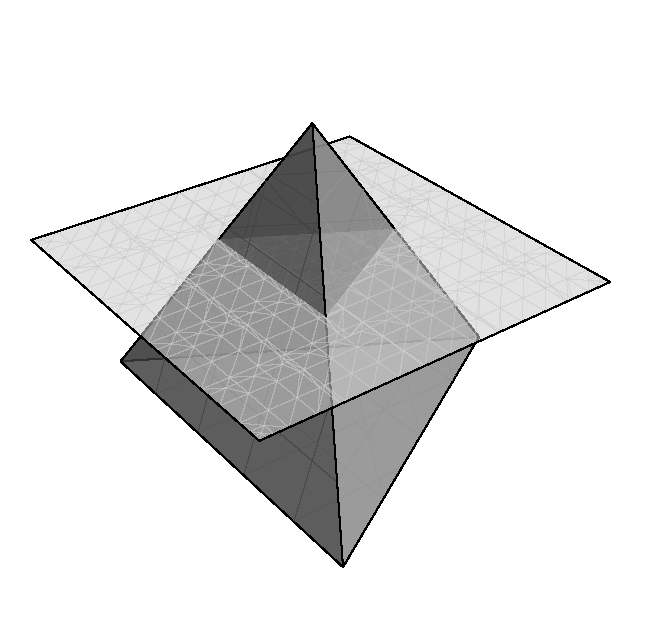
\includegraphics[scale=.5]{../graphics/planeCross.pdf}
\]
We're going to build a triangular-based pyramid out of numbers. Here
are the first four cross sections:
\[
1 \qquad 
\begin{tabular}{@{\,}c@{\,}c@{\,}c@{\,}}
1 & & 1\\
 & 1 & 
\end{tabular}
\qquad 
\begin{tabular}{@{\,}c@{\,}c@{\,}c@{\,}c@{\,}c@{\,}}
1 & & 2 & & 1 \\
 & 2 & & 2 &  \\
 & & 1 & &  
\end{tabular}
\qquad
\begin{tabular}{@{\,}c@{\,}c@{\,}c@{\,}c@{\,}c@{\,}c@{\,}c@{\,}}
1 & & 3 & & 3 & & 1 \\
 & 3 & & 6 & & 3 &  \\ 
 & & 3 & & 3 & &  \\ 
 & & & 1 & & &  
\end{tabular}
\]
This pyramid that we are building is called \textbf{Pascal's
  pyramid}.\index{Pascal's!pyramid}

\begin{prob} 
Give the next two cross sections of Pascal's pyramid. Explain your
reasoning.
\end{prob}


\begin{prob} 
Do you see any connections to Pascal's Triangle in Pascal's pyramid?
Explain what you see.
\end{prob}


\begin{prob} Use the Binomial Theorem to expand:
\[
(a + x)^3
\]
\end{prob}



\begin{prob} 
Replace $x$ above with $b+c$, and use the Binomial Theorem again along
with your computation above to expand:
\[
(a + b + c)^3
\]
\end{prob}


\begin{prob} 
What do you notice about the coefficients in the expansion of $(a + b + c)^3$?
\end{prob}


\begin{prob} Explain how the trinomial coefficient
\[
\binom{n}{j,k} = \frac{n!}{j! k!(n-j-k)!}
\]
corresponds to entries of Pascal's pyramid. Feel free to draw diagrams
and give examples.
\end{prob}

\begin{prob} 
The trinomial coefficient $\binom{n}{j,k}$ has the following
``physical'' meaning: It is the number of ways one can choose $j$
objects and $k$ objects from a set of $n$ objects. Try a couple of
relevant and revealing examples to provide evidence for this claim.
\end{prob}

\begin{prob}  
Explain how Pascal's Triangle is formed. In your explanation, use the
notation $\binom{n}{j,k}$. If you were so inclined to do so, could you
state a single equation that basically encapsulates your explanation
above?
\end{prob}


\begin{prob} 
Use Pascal's pyramid to expand:
\[
(a + b + c)^4
\]
Try to formulate a ``Trinomial Theorem.''
\end{prob}

\begin{prob} Use your Trinomial Theorem to explain why the numbers in the $n$th cross section of Pascal's pyramid sum to $3^n$.
\end{prob}

%%%%%%%%%%%%%%%%%%%%%%%%%%%%%%%%%%%%%%%%%%%%
%%%%%%%%%%%%%%%%%%%%%%%%%%%%%%%%%%%%%%%%%%%%
%% REF - R. L. Keeney and James F. Ramaley
%% Mathematics Magazine, Vol. 42, No. 4 (Sep., 1969), pp. 210-213 
%%
